\section{Website Structure}\label{sec:websitestructure}
The website is structured with a modified MVC pattern, for an explanation of the general idea of MVC see \secref{sec:mvc}.
In order to make the usage of MVC easy, a framework from \citep{misc:mvc-framework} is used.

The framework provides a \texttt{controller} base class, see \figref{fig:websitestructure}, which the new controllers inherit from, mainly providing a database instance.
It also provides an \texttt{Application} class that hand\-les URL parsing and navigation to the correct pages based on the URL.
In addition to this, it provides a directory structure. As an example, you can add a controller to the controller directory, and the \texttt{Application} class is able to load them, same idea goes for the model and view layer.

\begin{figure}[h]
	\centering
	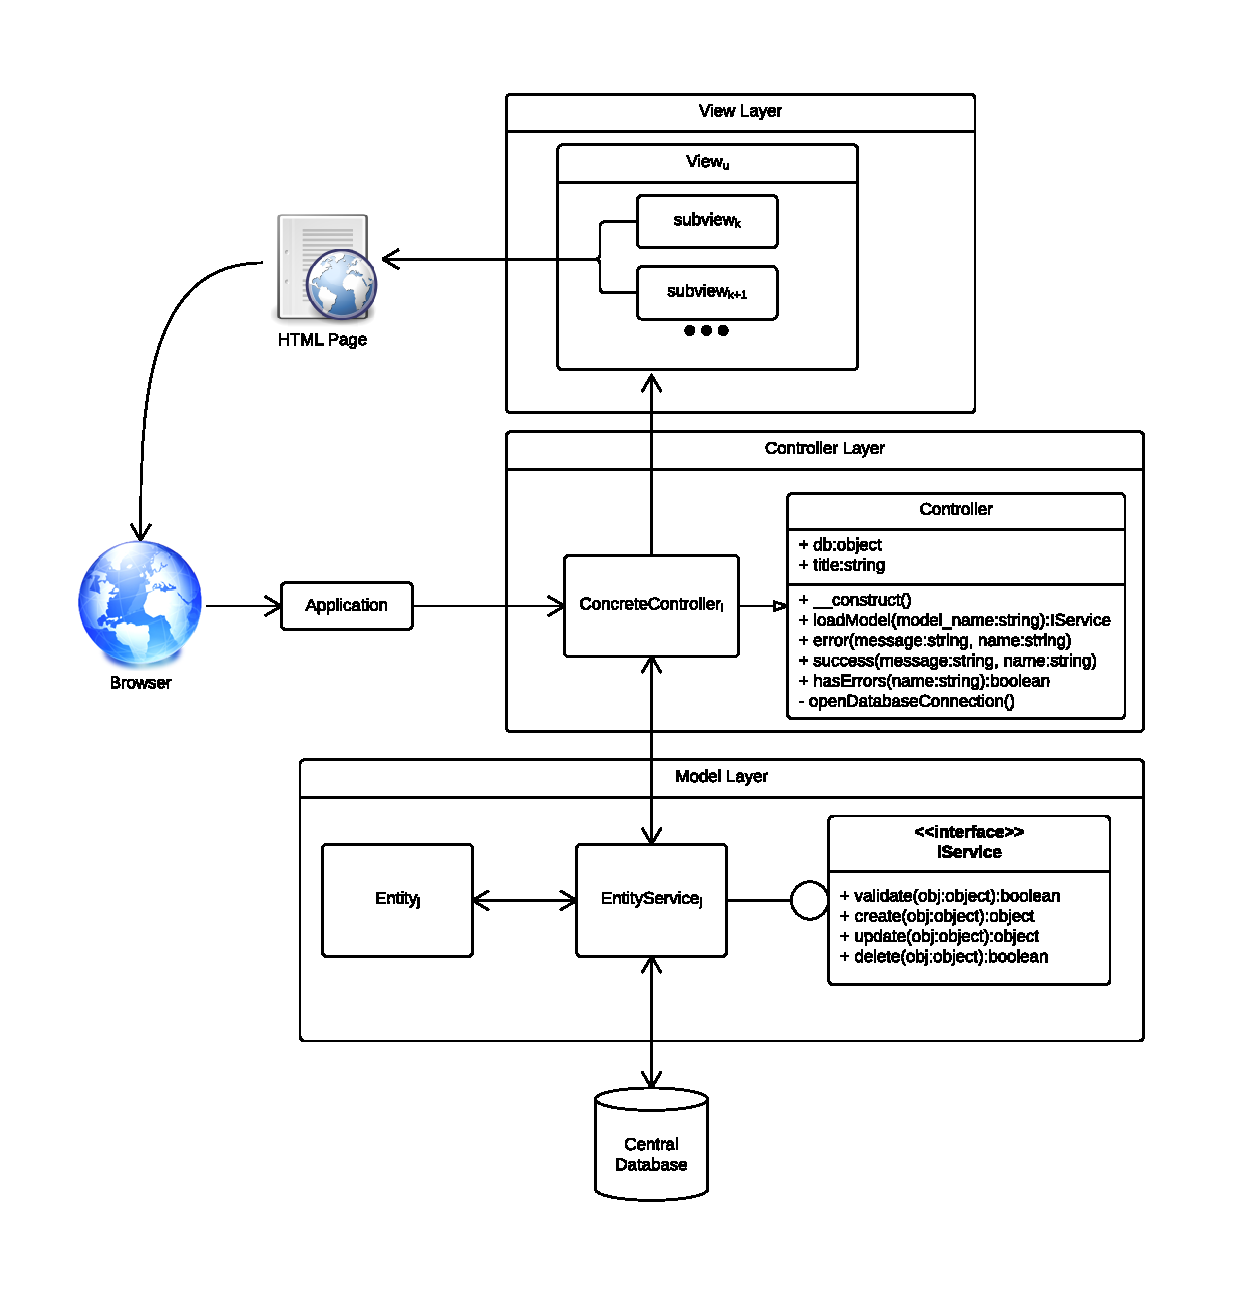
\includegraphics[scale=0.7, trim= 1cm 1.5cm 1.5cm 1.5cm, clip]{implementation/ConcreteMVC}
	\caption{Website Structure.}\label{fig:websitestructure}
\end{figure}

With inspiration from the MVC pattern and usage of the framework, the website was then structured as seen in \figref{fig:websitestructure}.
The idea of the figure is to represent the structure, where we abstract from concrete entity, view, and controller names, and instead denote these with the names $\texttt{Entity}_\texttt{j}$, $\texttt{EntityService}_\texttt{j}$, $\texttt{ConcreteController}_\texttt{i}$, and $\texttt{View}_\texttt{u}$.
The structure is split into several parts, each of which is examined in turn. 

\begin{description}[style=nextline]
	\item[Model Layer] 
	If you take a look at the \texttt{Model} layer, it is split into three parts, $\texttt{Entity}_\texttt{j}$, $\texttt{EntityService}_\texttt{j}$ and \texttt{iService}.
	$\texttt{Entity}_\texttt{j}$ is a wrapper class, which is used to encapsulate a row from a table in the database.
	$\texttt{EntityService}_\texttt{j}$ is then a service, implementing the CRUD methods of \texttt{iService}, thought of when determining the design, read is excluded from the interface because the number of parameters needed varies.
	$\texttt{EntityService}_\texttt{j}$ is what part of the model that is responsible for establishing the connection to the database, and enables the controller to work on the model, via calling the CRUD methods of the service, when a read method is called from a controller, an entity, or a list of entities representing the row(s) is then what is returned.
	The reason we differentiate between  $\texttt{Entity}_\texttt{j}$ and $\texttt{EntityService}_\texttt{j}$ is that we find it makes sense to differentiate between the data and the methods working on the data.
    Furthermore it provides a separation of responsibility from the \texttt{Entities} and the \texttt{EntityServices}, given that \texttt{Entities} provide a means of representing an entity of the database and that \texttt{EntityServices} provide the behaviour for those representations.
	
	\item[Controller Layer]
	The \texttt{Controller} layer consists of a number of controllers, $\texttt{ConcreteController}_\texttt{i}$, each of which inherits from a base \texttt{Controller} class, which provides functionality to load the model as well as registering successes and errors to be displayed to the user.
	Each concrete controller then contains a number of methods, corresponding to different pages, these methods are also called actions. 
    The responsibility of the concrete controller is then to work on the \texttt{model} and include \texttt{views}. 
	
	\item[View Layer]
	The \texttt{View} layer has the responsibility of presenting the data, prepared by the \texttt{controller}, to the user in a readable manner.
	
	In other words, the \texttt{View} layer takes care of the HTML generation part of the website, where each complete view in this context is considered a complete HTML page possibly consisting of various \texttt{subviews}.
	Some of the \texttt{subviews} reoccur in multiple complete views.
    Different classes of \texttt{subviews} exist, normal \texttt{subviews} and templates that are used almost universally throughout the website, for example the header and footer \texttt{subviews}.
	The combination of these \texttt{subviews} forms a complete \texttt{view} which constitute a HTML page to be provided to the browser.
	
	A characteristic of views in general is that it consist of a lot of HTML markup and a low amount of program logic, as this work is delegated to the model and controller layer. 
	
	\item[Application]
	When the browser visits the website, rewrite rules has been set in the \texttt{.htaccess} file, to ensure that the relative path part of the URL is given as an argument to the default index file. This index file then loads the required files, such that the instantiated Application object has access to the configuration files needed.
	The GET variable URL, which was set from the \texttt{.htaccess} file is then used by the Application object to navigate to the correct controller and action.
	
	
\end{description}

For a more detailed look at the model and controller layer, see \appref{app-arch:controller} and \appref{app-arch:model}.